\chapter{Конструкторская часть}

В данном разделе будут приведены схемы алгоритма полного перебора и муравьиного алгоритма для решения задачи коммивояжера, приведено описание используемых типов данных, классов эквивалентности, а также описаны исходные файлы программы.

\section{Алгоритмы решения задачи коммивояжера}

На рисунках \ref{fig:ant_alg_scheme} -- \ref{fig:full_comb_alg_scheme} приведены схемы алгоритмов для решения задачи коммивояжера (полного перебора и муравьиного алгоритма).

\begin{figure}[h]
	\centering
	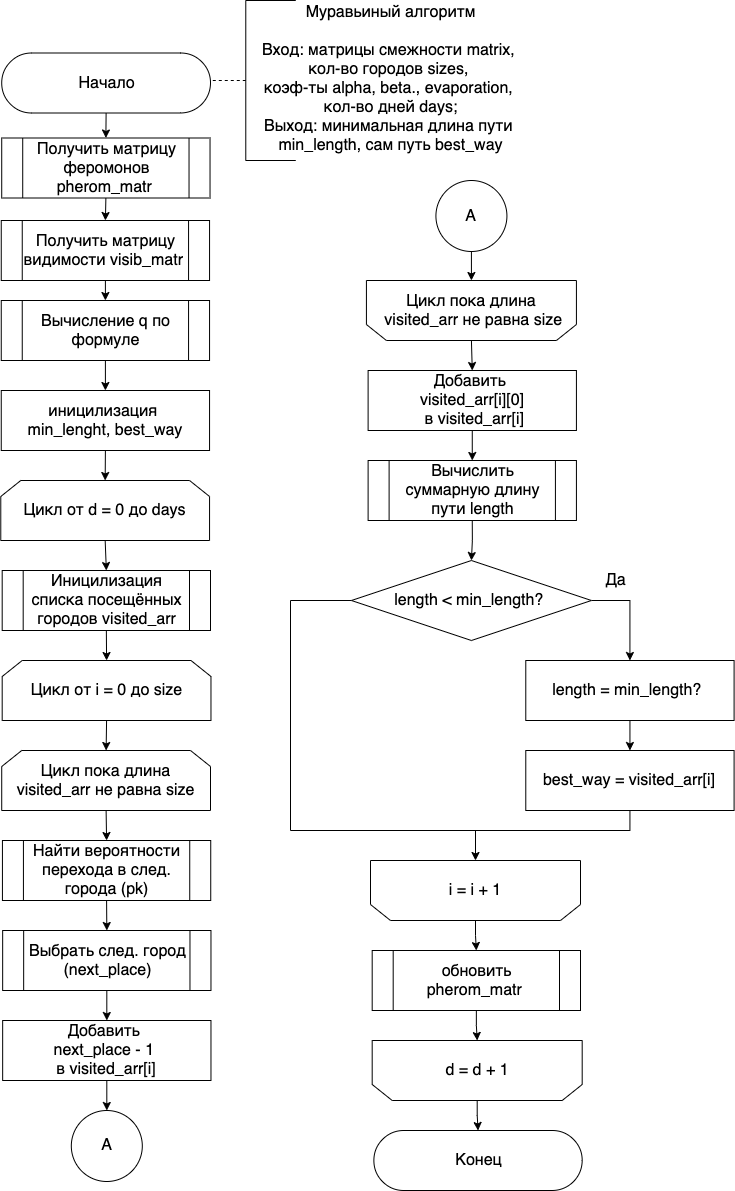
\includegraphics[scale=0.55]{img/ant_alg_scheme.png}
	\caption{Схема муравьиного алгоритма}
	\label{fig:ant_alg_scheme}
\end{figure}

\clearpage

\begin{figure}[h]
	\centering
	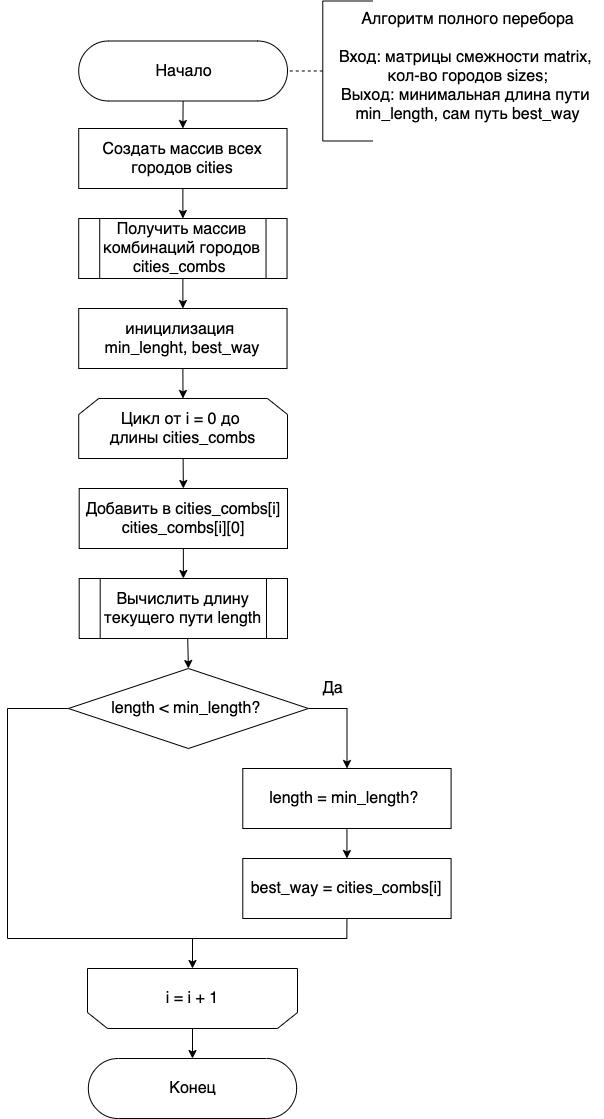
\includegraphics[scale=0.6]{img/full_comb_alg_scheme.png}
	\caption{Схема алгоритма полного перебора}
	\label{fig:full_comb_alg_scheme}
\end{figure}

\section{Описание типов данных}

При реализации алгоритмов будут использованы следующие структуры данных:

\begin{itemize}[label=---]
	\item размер матрицы смежности --- целое число типа $int$;
	\item матрица смежности --- матрица, элементы которой имеют тип $int$;
	\item коэффиценты $\alpha$, $\beta$, $evaporation$ --- действительные числа типа $float$;
	\item название файла --- строка типа $str$.
\end{itemize}

\clearpage

\section{Исходные файлы программы}

Программа будет состоять из следующих модулей:

\begin{itemize}[label=---]
	\item $main.py$ --- файл, содержащий функцию $main$;
	\item $generate.py$ --- файл, содержащий функцию для генирации матриц;
    \item $ant\_algorythm.py$ --- файл, в котором содержатся функции муравьиного алгоритма для решения задачи коммивояжера;
    \item $full\_combinations.py$ --- файл, в котором содержатся функции алгоритма полного перебора для решения задачи коммивояжера;
    \item $parametrization.py$ --- файл, содержащий функцию параметризации для муравьиного алгоритма;
    \item $compare\_time.py$ --- файл, в котором содержатся функции для замера времени работы алгоритмов и построения графика зависимоти времени выполнения от размера матрицы;
    \item $read\_print.py$ --- файл, в котором содержатся функции ввода вывода данных;
    \item $color.py$ --- файл, который содержит переменные типа $string$ для цветного вывода результата работы программы в консоль.
\end{itemize}

\clearpage